%%% Page couverture avant. Il faut modifier la largeur des graphiques
%%% puisque Sweave la règle à 0.8\textwidth.
\setkeys{Gin}{width=\paperwidth}
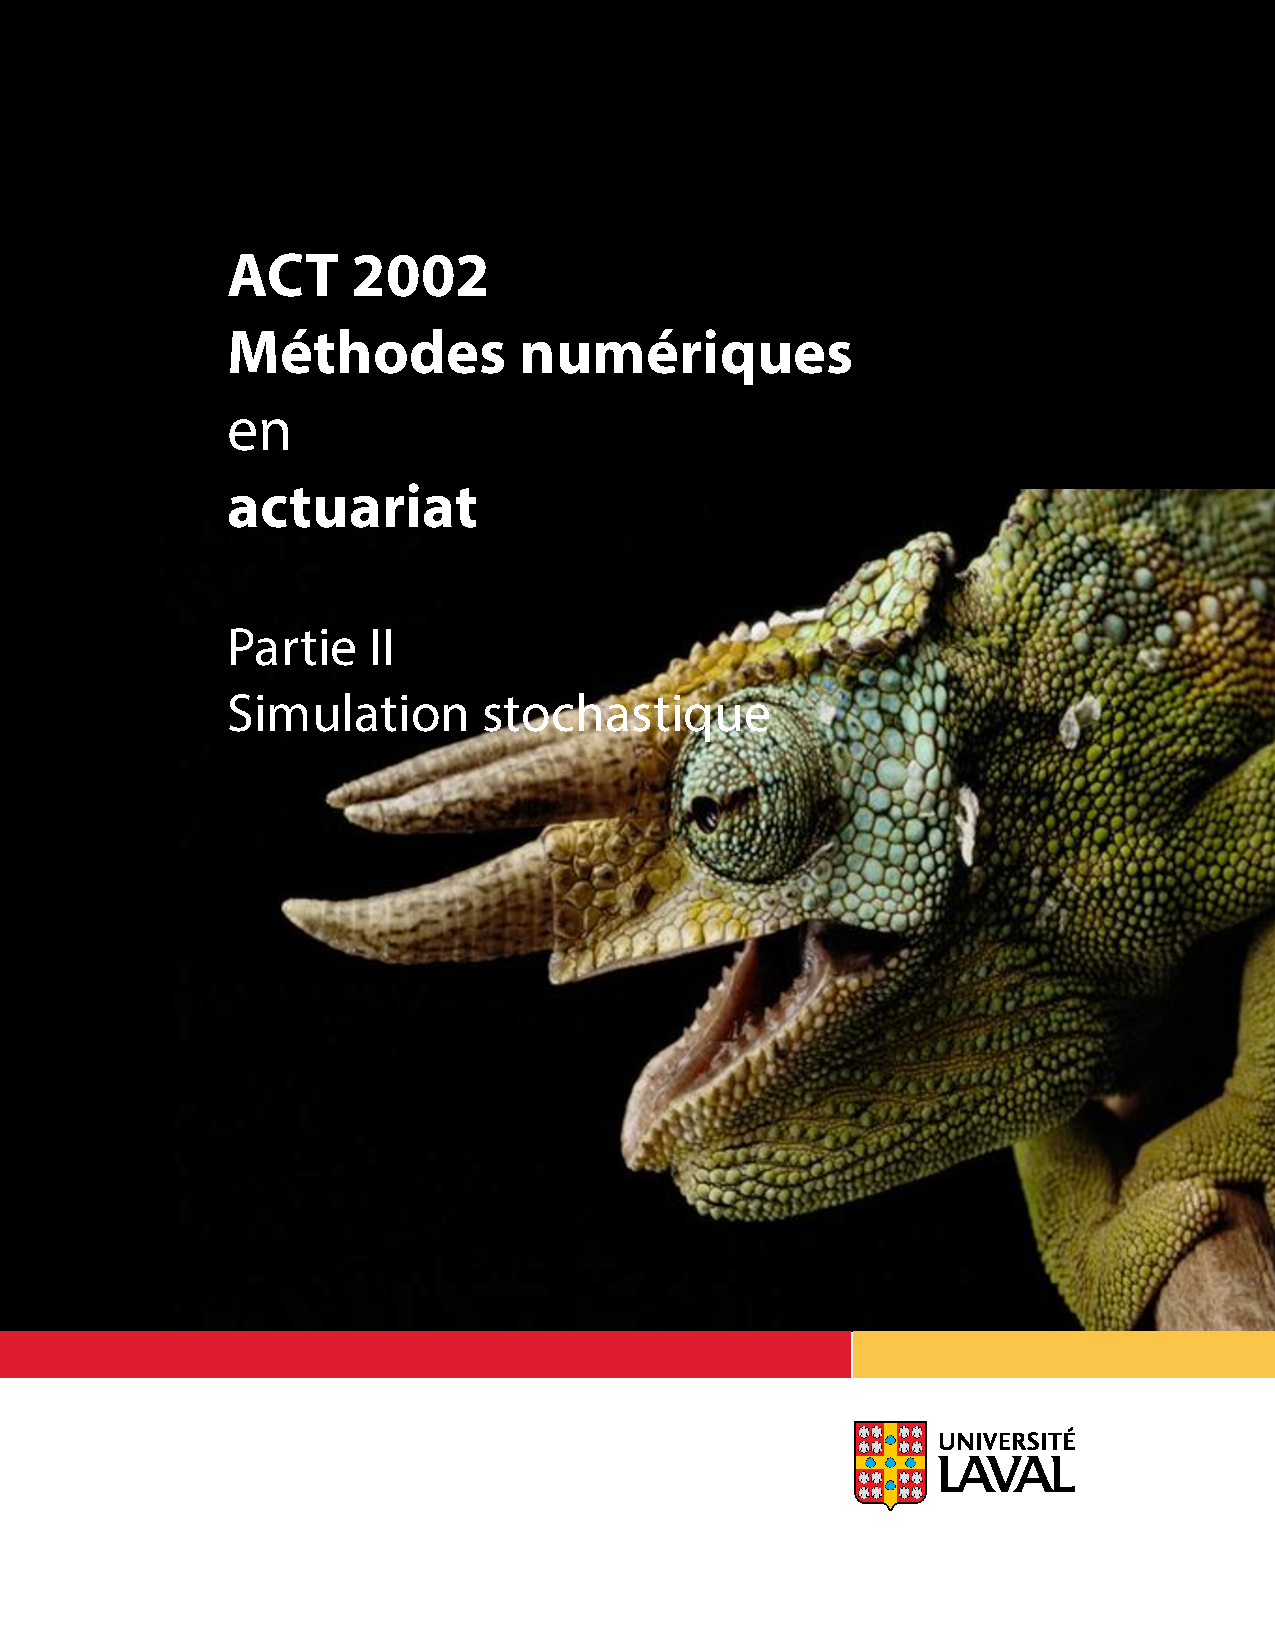
\includepdf[pages=1]{couvertures-partie_2}
\setkeys{Gin}{width=0.8\textwidth}

\cleardoublepage

%%% Page de garde
\begin{adjustwidth*}{13.1mm}{-72mm}
  \sffamily
  \raggedright
  \vspace*{5mm}
  \thetitle \\
  \vspace*{3cm}
  \theauthor \\
  \vspace*{\fill}
  \thedate
\end{adjustwidth*}
\clearpage

%%% Page de notices
\begingroup
\calccentering{\unitlength}
\begin{adjustwidth*}{\unitlength}{-\unitlength}
  \small
  \setlength{\parindent}{0pt}
  \setlength{\parskip}{\baselineskip}

  {\textcopyright} 2012 Vincent Goulet \\

  \includegraphics[height=7mm,keepaspectratio=true]{cc}\;%
  
\includegraphics[height=7mm,keepaspectratio=true]{by}\;%
  
\includegraphics[height=7mm,keepaspectratio=true]{sa} \\
  Cette création est mise à disposition selon le contrat
  Paternité-Partage à l'identique 2.5 Canada disponible en ligne
  \url{http://creativecommons.org/licenses/by-sa/2.5/ca/} ou par
  courrier postal à Creative Commons, 171 Second Street, Suite 300,
  San Francisco, California 94105, USA.

  \textbf{Code source} \\
  Le code source {\LaTeX} de ce document est disponible à l'adresse
    \url{https://svn.fsg.ulaval.ca/svn-pub/vgoulet/documents/methodes_numeriques/}
  ou en communiquant directement avec l'auteur.

  La photo de la couverture est tirée du site de National Geographic.
\end{adjustwidth*}
\endgroup

\clearpage

%%% Local Variables:
%%% mode: latex
%%% TeX-master: "methodes_numeriques-partie_2"
%%% End:
